\section*{Abstract}

Parasite exploitation after the emergence of parasite in a new host population leads to parasite (and host) evolution on ecological time scales. Yet, most models for parasite evolution are either restricted to long term evolution or assume that parasite fitness is defined only by virulence and transmission, which means that parasites always reside on their optimization frontier. This is an unrealistic assumption for any organism in a new environment. We present a model for the evolution of a parasite that is initially beneath its tradeoff frontier using a second quantitative trait that represents investment in ``compensatory'' traits (e.g. secondary virulence factors), which is required for parasites to effectively translate virulence into transmission. We analyze our model using three different approaches: a finite population, discrete time stochastic simulation-based model (DTS), a deterministic reaction-diffusion (differential equation based) model (RD), and an adaptive dynamics model (AD). Using these three models we aim to understand the effects of small populations and stochasticity on transient evolution, time to the adaptive peak, and periodic departures of the population from its adaptive peak. We find that the RD and DTS models show qualitatively similar patterns across a range of parameter values and starting conditions, though these patterns begin to diverge as host populations become very small. We show that with an adaptive landscape with a single maximum, an AD also provide an adequate description qualitative description of parasite evolutionary dynamics. In all three models parasites evolve higher than optimal virulence in the short term because of the negative fitness effects of a mismatch between replication rate and compensatory virulence factors. Eco-evolutionary dynamics also contribute to higher transient virulence in the RD and DTS models. In simple evolutionary models we find that a DTS model may be unnecessary; simple RD or AD models are sufficient to understand parasite qualitative evolutionary dynamics. However, if rare evolutionary events in small populations are of primary interest, only the DTS model is appropriate. 

\subsection*{Keywords:}
Adaptive Dynamics; Parasite Exploitation; Reaction Diffusion; Stochastic Simulation; Tradeoff theory 

\clearpage
\doublespacing

\section*{Introduction}

Parasite exploitation of their host exerts strong selection pressure on both parasite exploitation strategy and host defense strategy \citep{SchneiderandAyres2008, AyresandSchneider2012, KutzerandArmitage2016}. The resulting evolution often occurs at ecological time scales \citep{DayandProulx2004, Bolkeretal.2010, Lion2018}, and sometimes in a predictable way \citep{Ebert1998, Pugliese2002, Laineetal.2008, Frickeletal.2016}. Often, rapid evolution occurs after a parasite jumps species or emerges in a new host populations; examples of rapid parasite evolution following invasion include: WNV in North American birds \citep{Beasleyetal.2003}, MYXV in Eurpoean rabbits \citep{FennerandMarshall1957}, \emph{Plasmodium falciparum} in House finches \citep{Flemingetal.2018}, HIV in Humans \citep{Fraseretal.2007}, $\lambda$ phage in \emph{E. coli.} \citep{Berngruberetal.2015}, \emph{phycodnaviridae} family dsDNA viruses in algae \citep{Frickeletal.2016, Frickeletal.2018}, and \emph{Pasteuria ramosa} in \emph{Daphnia sp.} \citep{Duffyetal.2009}. 

In the past four decades, models for parasite evolution informed by these examples have revealed generalities in parasite evolution and helped to explain parasite exploitation strategy in specific systems \citep[for a review see][]{Cressleretal.2016}. However, most of these models are restricted to long term evolution despite common rapid evolution \citep[but see][]{Bolkeretal.2010, Lion2018, Parsonsetal.2018}. Models often also collapse high-dimensional host-parasite interactions to two axes: parasite virulence (the rate of host mortality) and parasite transmission rate, which jointly determine parasite fitness \citep{AndersonandMay1982, Ewald1983, AlizonandMichalakis2015, Cressleretal.2016}. These choices result in a model where parasites move only \emph{on} their optimization frontier, which is unrealistic for any organism in a new environment. In this paradigm it is impossible to understand how a parasite evolves \emph{to} this frontier because parasite traits apart from virulence and transmission are taken as a ``black box'' \citep{Alizonetal.2009, BullandLauring2014, AlizonandMichalakis2015}.

While it is relatively common for models to extend tradeoff theory using additional axes of complexity such as within-host parasite dynamics \citep{AlizonandvanBaalen2005, Dayetal.2011, Mideoetal.2011}, host evolution \citep{CarvalandFerriere2010, Bestetal.2014, Papkouetal.2016}, or spatial structure \citep{Lipsitchetal.1995, HaraguchiandSasaki2000, LionandGandon2015}, we are unaware of a model that helps to explain parasite evolution both to and on the tradeoff curve by treating the tradeoff curve as a true \emph{optimization frontier}. \citet{Alizonetal.2009} mention in passing that parasites beneath their frontier will first evolve to their frontier and then to the tradeoff optimum; however, no additional discussion is given here, or to our knowledge elsewhere, on the evolutionary trajectory a parasite takes to reach its global optimum while under the constraint of tradeoff between virulence and transmission. 

Here we present a model for the evolution of a parasite that is initially beneath its tradeoff frontier when it invades a new host population. Our model introduces a second trait axis, in addition to the commonly used virulence, on which parasites evolve: a quantitative trait representation of investment in ``compensatory'' traits (e.g. secondary virulence factors) that affect the ability of a parasite to efficiently translate virulence into transmission. In classic tradeoff theory, a change in parasite virulence results in a correlated change in transmission following an assumed tradeoff curve function (often either a power-law or sigmoidal function: \citealt{AlizonandvanBaalen2005, Bolkeretal.2010, Kainetal.2018}). However, an increase in parasite replication rate may only lead to an increase in transmission rate following changes in other genes. For example, changes to the MYXV virulence factor M148R, which helps to downregulate the host immune system, are needed for an increase in MYXV replication rate to increase transmission, because a secondary side effect of an increased replication rate is a more rapid upregulation of the host immune system \citep{Blanieetal.2009}. Even in the absence of host immune regulation, it is not difficult to imagine that an increase in investment in replication rate, for example, leads to a decrease in \emph{per capita} infection efficiency, enough that \emph{total} efficiency decreases, because of a quantity vs quality life-history tradeoff. To recover this \emph{per capita} efficiency and further increase total efficiency, adjustments in secondary traits are needed. While it is conceivably possible to model the evolutionary dynamics of multiple individual virulence factors, to our knowledge no system is simple enough nor is enough known currently about the function of all of the protein products of a specific parasite for this approach to be fruitful. 

Models of parasite evolution often also assume both deterministic evolution in an infinite population and a separation of ecological and evolutionary time scales, despite strong evidence that parasite exploitation affects host population size which influences evolution on ecological time scales \citep{Frickeletal.2016, Papkouetal.2016, Frickeletal.2018}. These assumptions make it impossible to study rapid evolution following parasite emergence, or as a result of environmental fluctuations such as seasonality (however, see \citealt{DayandProulx2004}, \citealt{Bolkeretal.2010}, \citealt{Lion2018}, and \citealt{Parsonsetal.2018}). These simplifications are often made in order to obtain analytic solutions, which are usually more easily generalizable; solutions from stochastic simulations are likely to be tied more closely to specific systems and can potentially lead to less powerful conclusions. However, because many researchers have recently been calling for more of a case-study approach \citep{BullandLauring2014, AlizonandMichalakis2015, Cressleretal.2016}, a reduced ability to make widely generalizable conclusions may be a minimal drawback. Work on evolution in finite populations is also restricted by a lack of mathematical theory for deriving analytic solutions for evolution in finite populations on ecological time scales \citep{Lion2018}, though \citet{Parsonsetal.2018} have recently derived analytic solutions for parasite evolution in finite populations using \emph{Stochastic Adaptive Dynamics}. While this model more closely resembles parasite evolution in practice, it assumes rare and small-effect mutations which are unlikely for at least viral pathogens (e.g. MYXV, WNV, \emph{phycodnaviridae} dsDNA viruses). 

We analyze our model for the mechanics of parasite exploitation using three different modeling approaches: a biologically realistic scenario of parasite evolution in finite populations using a discrete time stochastic simulation-based model, as well as a deterministic reaction-diffusion (differential equation based) model (RD) that captures both selection (advection) and mutation (diffusion) and an adaptive dynamics representation of the problem (AD). These deterministic approaches serve as two forms of ``null-models'' against which we compare the results of our stochastic model. Using these three models we aim to understand the effects of small populations and stochasticity on transient evolution, time to the adaptive peak, and periodic departures of the population from its adaptive peak. We examine when and what interesting biological patterns emerge as a function of increasing model complexity; that is, what we can learn about parasite evolution using a stochastic model that is missed when using a simpler framework.

\section*{Methods}

We examine a parasite that is constrained by a tradeoff between virulence and transmission \citep{AndersonandMay1982, Ewald1983}, where transmission rate ($\beta$) is an increasing function of host mortality rate (virulence: $\alpha$). When $\beta$ is a convex function of $\alpha$ ($\frac{\partial^2 \beta}{\partial \alpha^2} < 0$), a single intermediate value of $\alpha$ maximizes $\rzero$ \citep{Alizonetal.2009}. Here we use a power-law function to model the relationship between $\alpha$ and $\beta$ \citep{AlizonandvanBaalen2005, Bolkeretal.2010}: 
\begin{equation*}
\beta(\alpha) = c\alpha^{\frac{1}{\rho}},
\end{equation*}

\noindent where $\rho$ controls the function's curvature and $c$ is a scaling factor. For a power-law function, $\rzero$ is given by:

\begin{equation*}
\rzero = \frac{c\alpha^{\frac{1}{\rho}}}{\mu + \alpha + \gamma}
\end{equation*}

\noindent where $\mu$ is the background rate of host mortality and $\gamma$ is the rate of host recovery. The $\rzero$ of a parasite constrained by only a power-law tradeoff is obtained at $\alphastar = \frac{\mu + \gamma}{(\rho - 1)}$ \citep{Bolkeretal.2010, Kainetal.2018}. 

Here we model parasite transmission that is controlled by both replication rate and a trait that we call ``tuning'', which we take as a collective representation of the status of a collection of ``compensatory'' secondary virulence factors. For example, an increase in investment in replication rate could lead to a decrease in parasite \emph{per capita} efficiency; to recover and/or increase \emph{total} efficiency, adjustments in secondary virulence factors are needed. In general, we imagine that an appropriate level of investment in compensatory traits is what allows a parasite to realize maximum transmission at a given replication rate. 

We define $\beta$ given by the power-law tradeoff as the frontier (i.e. maximum achievable) transmission rate ($\betaf$) that is obtained when parasite tuning is perfectly matched to replication rate. The actual transmission rate of a parasite, realized transmission rate $\betar$, is a decreasing function of the mismatch between replication rate and tuning. We calculate $\betar$ as $\betaf$ multiplied by parasite efficiency ($\omega$), which is given by:

\begin{equation}
\omega = e^{\frac{-(\phi - \theta)^2}{\delta}},
\end{equation}

\noindent where log(replication rate) is given by $\phi$, tuning by $\theta$, and $\delta$ is a scaling factor (which we call the efficiency scale) that determines the cost of a mismatch between $\phi$ and $\theta$. Thus, $\betar = \betaf * \omega$, where $\betar = \betaf$ occurs only when $\phi = \theta$ (i.e. a perfectly tuned parasite). Because $\omega = 1$ when $\phi = \theta$, $\delta$ does not change the $\phi$ that optimizes $\rzero$, but does change $\rzero$ when $\phi \neq \theta$. In the limit of $\delta \rightarrow \infty$, the impact of $\theta$ on parasite fitness decreases to zero and the model collapses to classic tradeoff theory. In this model, parasite $\rzero$ is given by:

\begin{equation}
\omega \frac{\beta(\alpha)}{\alpha + \gamma + \mu}.
\end{equation}

While parasite fitness ($\rzero$) is defined by virulence ($\alpha$) and transmission ($\beta$), replication rate ($\phi$) and tuning ($\theta$) are the evolving traits. We model $\phi$ as the log or replication rate, and $\alpha$ as the inverse-logit of $\phi$ ($\alpha = \frac{e^{\phi}}{e^{\phi} + 1}$). We use a logistic scale for two reasons: First, the non-linear logistic scale is a convenient scale on which to model mutations that have little effect when a parasite has either a low or high trait value; second, the logistic scale maps the unbounded scale on which mutation occurs to (0, 1), which allows us to translate parasite replication rate and tuning to probabilities of transmission and host mortality for the DTS model.

In reality, parasite virulence and transmission are a joint function of parasite exploitation strategy and host defense strategy; following parasite invasion, parasite exploitation and parasite defense are known to co-evolve \citep{FennerandMarshall1957, CarvalandFerriere2010, Bestetal.2014}. To simplify the problem, we make the unrealistic assumption of no host evolution, and instead assume a static level of total host defensive capabilities. While we do not model host defenses, they are in a sense intrinsically captured in our model through parasite tuning. That is, a change in parasite replication rate can be imagined to lead to an initial decline in transmission because of increased host immune efficiency, at which parasites must ``retune'' to maximize transmission (similar to what has been seen in MYXV).

Using these definitions for parasite exploitation and fitness, we examine parasite evolution using three common modeling techniques: a discrete time, stochastic, finite population model (DTS), a reaction-diffusion, differential equation model (RD) and an adaptive dynamics (AD) model. Our primary interest is on stochastic evolutionary dynamics in small populations; however, results from stochastic simulation can be difficult to interpret on their own. We use results from the RD model, which is deterministic and assumes an infinite population, but which allows for eco-evolutionary feedbacks, as well as the AD model which assumes a separation ecological and evolutionary time scales, and small-effect mutations, to examine the effects of small populations and stochasticity on transient evolution, time to the adaptive peak, and periodic departures of the population from its adaptive peak. We begin with a description of the DTS model and then describe the simplified RD and AD models.

\subsection*{Discrete time, stochastic, finite population model (DTS)}

We model parasite transmission using an SISD model, defined by three host classes: Susceptible (S), infected (I), and dead (D). Infected hosts either recover from infection, at which point they become susceptible, or die and become removed from the population. We assume a homogeneous host population. A unique parasite strain is defined as a strain with a different value for replication rate and/or tuning, and thus virulence and transmission.

In each time step of the DTS model the following events occur: S and I hosts die with background mortality probability $\mu$; I hosts die with probability equal to the virulence of the strain they are infected with; S and I hosts reproduce in a density dependent manner, where the probability of reproduction is equal to one minus the ratio of the sum of living S and I hosts to the starting population size if the population size is less than the initial population size and zero otherwise; Infected hosts recover with probability $\gamma$ (hosts were assumed to have the same recovery rate from infection for all parasite strains; for the evolution of recovery see \citealt{AndersonandMay1982, AlizonandvanBaalen2005}); and S hosts become infected. A proportion of S hosts \emph{escape} infection with probability equal to:

\begin{equation*}
\prod_{i} (1 - \beta_{i}),
\end{equation*}

\noindent while the susceptible hosts that do become infected are infected with strain \emph{i} with probability \emph{approximately} equal to:

\begin{equation*}
p_{i} = \frac{n_{i}R_{0i}}{\sum_{j}n_{j}R_{0j}}.
\end{equation*}

Using probabilities instead of rates for transmission, death, and recovery leads to a slightly modified equation for $\rzero$ of:

\begin{equation}
\rzero = \omega \frac{c\alpha^{\frac{1}{\rho}}}{1 - ((1 - \mu)(1-\alpha)(1-\gamma))}.
\end{equation}

\noindent This equation leads to a slightly higher level of optimal virulence than for Eq.2 when using the same parameter values for $\mu$ and $\gamma$. 

We assume a mutation occurs in parasite strain \emph{i} during transmission with probability $\pi$, and that mutations have an additive effect on the logistic scale. Mutational effect sizes for both traits are drawn from a multivariate Normal distribution with a mean of zero, positive standard deviation (the same value for $\sigma$ was used for both traits), and zero covariance. That is:

\begin{equation*}
\left.\begin{matrix}
 & \phi_{i} \rightarrow \phi_{i} + MVN(0, \Sigma_{1,1})  \\ 
 & \theta_{i} \rightarrow \theta_{i} + MVN(0, \Sigma_{2,2}) 
\end{matrix}\right\} | B(1, \mu) = 1
\end{equation*}

Newly birthed and recovered hosts are not available to be infected until the next time step and newly infected hosts cannot die, recover, or infect S hosts until the next time step. This process proceeds for a specified length of time or until all hosts or all parasites go extinct. 

\subsection*{Reaction diffusion model}

The model described above can be written using a system of differential equations, using rates instead of probabilities:

%\begin{equation*}
\begin{align*}
& \frac{\mathrm{d} S}{\mathrm{d} t} = bS - \mu S - S \int_{0}^{\infty}  \int_{0}^{\infty} \beta(\alpha(\phi, \theta, t)))i(\phi, \theta, t)d\phi d\theta + \gamma \int_{0}^{\infty}  \int_{0}^{\infty} i(\phi, \theta, t)d\phi d\theta \\ 
& \frac{\partial i}{\partial t} = [S\beta(\alpha(\phi, \theta, t)) - (\alpha + \mu + \gamma)]i(\phi, \theta, t) + D\frac{\partial^2 i}{\partial \phi^2} + D\frac{\partial^2 i}{\partial \theta^2},
\end{align*}
%\end{equation*}

\noindent where the second derivative (diffusion) terms model the mutational process in replication rate and tuning. To remove the integrals in these equations to efficiently solve this system, we discretized replication rate and tuning into an \emph{m x m} matrix. Each cell of this matrix represents a combination of trait values, and the number in each cell representing the number (proportion) of individuals infected with a strain with that combination of trait values. Diffusion on this matrix represents mutation from one trait value to another, using constant step sizes on the logistic scale. We solved this system of differential equations using the {\tt ode} function in the {\tt deSolve} package \citep{Soetaertetal.2010} in {\tt R} \citep{Rcoreteam}; diffusion was implemented using the {\tt tran.2d} function in the {\tt ReacTran} \citep{SoetaertandMeysman2012} package using a zero-flux boundary condition (no loss of infected individuals due to mutation). 

\subsection*{Adaptive dynamics model}

When ecological dynamics are assumed to be fast relative to evolutionary dynamics (a new parasite mutant only invades at ecological equilibrium), and mutational effect size is small, it has been shown that parasites evolve to optimize $\rzero$ \citep{Dieckmann2002, KeelingandRohani2008, Lion2018}. By definition, once at ecological equilibrium a resident strain has an $\rzero = 1$. A new mutant is able to invade if it has an $\Reff > 1$ (a single host infected with a mutant strain infects greater than one new host at the equilibrium number of S set by the resident strain). In simple epidemiological models (e.g. SIS, SIR) \citep{Dieckmann2002, KeelingandRohani2008, Lion2018}, an $\Reff > 1$ corresponds to an $\rzero > 1$. Starting with an arbitrary resident stain, we allow mutant strains with $\Reff = 1 + \epsilon$ to invade and fixate until no new mutant strains have $\Reff > 1$. This process can be used to find the optimal parasite strategy, though it is not guaranteed that the optimum found is the global optimum \citep{Dieckmann2002}.

Our model generates a fitness landscape (we use this term to describe the relationship between parasite tuning, replication rate and $\rzero$) with a single global maximum and no local maxima for all parameter values. We implement AD by relying on the criteria that a mutant strain with $\rzero$ greater than the resident strain will displace the resident strain. Using mutations with the small additive effect of 0.005 on the logistic scale ($\phi_{t+1}$ = $\phi_t \pm 0.005$; $\theta_{t+1}$ = $\theta_t \pm 0.005$), we allow mutant strains to replace the resident strain until all mutants have an $\Reff < 1$. We consider parasite evolution when a parasite can have a simultaneous mutation in both replication rate and tuning (which we assume in both the DTS and RD models), or a mutation in only a single trait at a time. For the model with mutation in both traits it is possible that a number of mutational changes (e.g. an increase in replication rate and tuning vs an increase in replication rate but a decrease in tuning) can lead to a higher $\rzero$; we assume that the mutant parasite with the larger $\rzero$ invades, which removes any stochasticity from this model. That is, the invading strain, within the mutational range of $\pm \epsilon$ \emph{for both traits}, with the highest $\rzero$ displaces the resident (for a stochastic version of adaptive dynamics see \citealt{Parsonsetal.2018}).

\subsection*{Model outcomes}

Our primary aim is to understand the dynamics of the DTS model; we use the results from the RD and AD models to help us clarify the effects of stochasticity and small populations. We focus primarily on three outcomes: transient patterns in parasite virulence, the time it takes a parasite to reach its global optimum, and the size of the long-term virulence distribution (due to mutation/selection balance and/or stochastic departures from the global optimum). We ran all three models across a range of parameter values for $\mu$, $\sigma$, N, $\delta$, and initial tuning and replication rate (Table~1). We explore only a single power-law tradeoff. For our DTS model we used 250 stochastic simulations for each parameter combination.

\begin{table}[H]
\centering
\caption{Parameter values used in the DTS (discrete time, stochastic, finite population) RD (reaction-diffusion), and AD (adaptive dynamics) models. Parameter values that are not used in a given model are written as ``--''. Starting values for $\phi$ and $\theta$ for the RD model are closer to 0 on the logit scale because of numeric instability at more extreme starting conditions. Values for the power-law scaling parameter (\emph{c}) was increased in the RD model to insure an $\rzero > 1$ at extreme combinations of $\phi$ and $\theta$ with a $\delta$ of 10. An increase in \emph{c} increases $\rzero$ but does not affect the shape of the fitness surface. } \label{tab:model_details} 
\resizebox{\columnwidth}{!}{
\bgroup
\begin{tabular}[c]{|R{2.50cm}:R{4.00cm}:R{4.00cm}:R{4.20cm}|}
\hline
     \textbf{Parameter}        &
     \textbf{DTS model}        &
     \textbf{RD model}         & 
     \textbf{AD model} 	
\\
\hline
\rowcolor{vlg}
$\delta$     & 
10, 30, 50   &
10, 30, 50   &
10, 30, 50   
       
\\
$\mu$                                            & 
0.001, 0.005, 0.025                              &
--                                               &
1 or 2 mutations in each new mutant, 
occurs after ecological equilibrium is reached   
       
\\
\rowcolor{vlg}
Mutational $\Sigma$                        & 
0.05, 0.01, 0.25                           &
0.025 * 2.5\textsuperscript{0, 1, 2, 3}    &
Constant mutational size of 0.005          
       
\\
Population Size    & 
200, 600, 1800     &
--                 &
--                 
       
\\
\rowcolor{vlg}
Starting [$\phi$, $\theta$]                                                         & 
[logit(0.03), logit(0.97)], [logit(0.97), logit(0.03)], [logit(0.03), logit(0.03)]  & 
[logit(0.80), logit(0.20)], [logit(0.20), logit(0.80)], [logit(0.20), logit(0.20)]  &
[logit(0.03), logit(0.97)], [logit(0.97), logit(0.03)], [logit(0.03), logit(0.03)]  
       
\\
Power-law \emph{c} & 
0.75     &
2-20     &
0.75     
       
\\
     \rowcolor{vlg}
Power-law \emph{$\rho$} & 
2     &
2     &
2     
       
\\

\hline

\end{tabular}
\egroup
}
\end{table}

\clearpage


\section*{Results}

We first compare qualitative patterns in parasite evolution among the DTS, RD, and AD models for single parameter sets. We then describe the effects of each parameter on each of our metrics of interest in the DTS model. In all cases we focus on a scenario where a parasite evolves from an initial position of low replication rate and low efficiency (high tuning), which we use to represent a parasite that has recently jumped species and is poorly suited to its new host. In the online supplement we present results when a parasite evolves from high replication rate and low efficiency (another possible scenario following a species jump) (Figure~S1) as well as low replication rate, high efficiency (Figure~S2). We focus on patterns in parasite virulence and transmission, which are the observable traits from the point of view of an exploited host population. We focus less explicitly on tuning, which effects transmission and constrains virulence evolution but serves as a ``silent'' trait that is a step removed from epidemiology/ecology. 

\subsection*{Climbing the fitness landscape: qualitative patterns among models}

The RD and DTS models show qualitatively similar patterns when using similar parameter values for mutational variance in the DTS model and the strength of diffusion in the RD model ($\sigma$ in both models) (\figref{landscape1}). The medians of the RD and DTS models show similar patterns for a parasites' evolution in tuning and replication rate, despite marginal differences in the curvature of the fitness landscape, which occurs because of the difference in the equation for $\rzero$ when using rates or probabilities (see Figure S3 for a comparison of the landscapes). With a $\rho = 2$ in the power-law tradeoff curve, parasites maximize $\rzero$ at a virulence of 0.21 and 0.26 in the RD and DTS models respectively (\figref{landscape1}). Variation among stochastic runs also roughly match the size of the variation in the DTS model at these parameter values; however, these patterns describe somewhat different processes. The RD model describes variation within a population of parasites, while the DTS model variation pictured in \figref{landscape1} describes variation among stochastic realizations (we discuss variation within a single stochastic run in the following results section). Even so, \figref{landscape1} shows that the simpler RD model provides an adequate qualitative match to the DTS model dynamics.

The AD model results show that even though parasites overshoot their optimal virulence in the absence of ecological dynamics, parasites evolve to their optimum phenotype in a more direct route than in either the RD and DTS models (\figref{landscape1} bold black line). Eco-evolutionary feedbacks in the RD and DTS models select for increased $\beta$ in the short term \citep{DayandProulx2004, Bolkeretal.2010}, which results in higher transient virulence than in the AD model (\figref{landscape1}, top left panel). Selection for higher $\beta$ also leads to a positive feedback for higher $\beta$ (and therefore $\alpha$), because strains with higher $\beta$ mutate faster than strains with lower $\beta$. In AD, when mutations only occur in a single trait at a time (\figref{landscape1} bold black dashed line), a parasites evolves to its optimum level of virulence first, and then to its optimum level of tuning. This pattern is seen across a wide range of parameter values for $\delta$ and the shape of the tradeoff curve, including the parameters used in \figref{landscape1} (e.g. Figures S~1, S~2); a parasite evolving according to AD with mutations in single traits will evolve tuning first only with a small $\delta$ and flat power-law tradeoff curve (small $\rho$) (not pictured).

\begin{figure}[H]
\makebox[\textwidth][c]{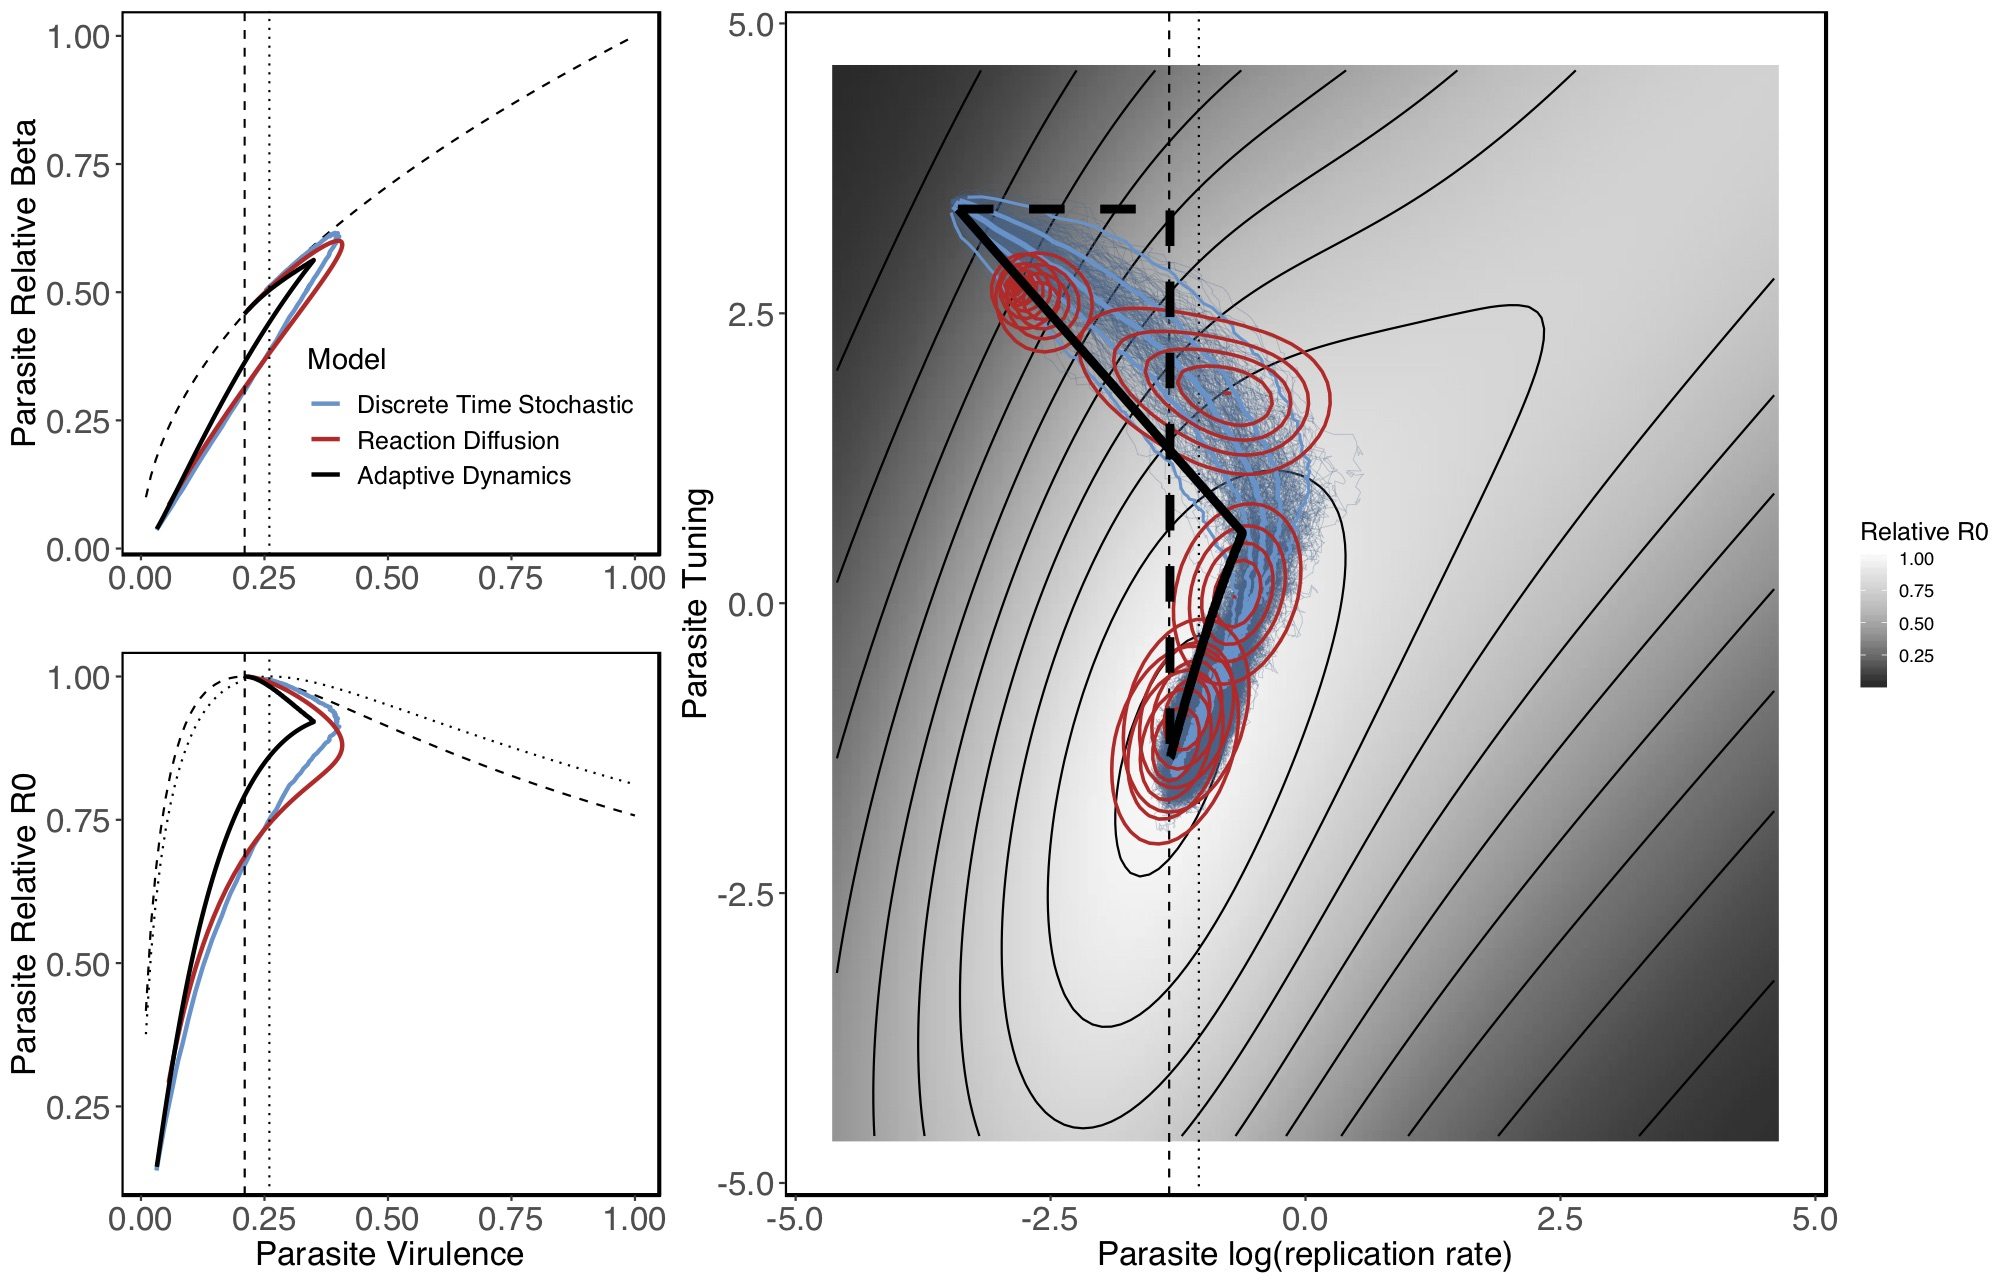
\includegraphics[width=1.0\textwidth]{Figures/landscape1.jpg}}
\caption{The large right panel shows the evolutionary trajectory of a parasite on its fitness landscape in the DTS model (thin blue lines show 250 stochastic simulations, while the solid blue lines show the median, 50\%, and 95\% quantities of these simulations), RD model (red ellipses show 95\% of the distribution of parasite strains), and AD model (bold black solid line shows simultaneous evolution in two traits; dashed lines show evolution in a single trait per time step), using the following parameter values: DTS: $\mu = 0.005$, $\sigma = 0.05$, N = 600; RD: $\sigma = 0.0625$; All models: $\delta = 30$. The surface pictured is calculated using the $\rzero$ equation for rates (Eq.2), and has been scaled so that the adaptive peak has a value of 1 (shown in light grey). Due to the slight difference in $\rzero$ for the RD and DTS models (Eq.2 vs Eq.3), the DTS surface is marginally different (see Figure~S3 for a comparison of these surfaces). The thin dashed vertical line shows the location of the adaptive peak for this surface; the thin dotted vertical line shows the location of the peak for the DTS model. 
\break
The top left and bottom left panels show a parasite evolving in log(replication rate) and tuning, according to the right panel, translated into virulence and transmission following a power-law tradeoff (top) and virulence and $\rzero$ (bottom). The dashed curve in the bottom left panel shows parasite $\rzero$ for the RD and AD models; the dotted curves shows parasite $\rzero$ for the DTS model. Maximum $\rzero$ is designated by the vertical dashed and dotted lines respectively. All models have the same power-law tradeoff curve (top). A numeric summary of the DTS model for these parameter values is available in Table~2 row~2.} 
\label{fig:landscape1}
\end{figure} 
\clearpage

A smaller efficiency scale ($\delta$) value increases the fitness cost of a mismatch between replication rate and tuning (Eq.1), which leads to higher parasite virulence in the short term in all models (\figref{landscape2}) (a larger $\delta$ decreases the cost, and leads to lower transient parasite virulence: \figref{landscape3}). Qualitative differences between the AD and RD/DTS models are similar across the range of values for $\delta$ used here (Figures~1-3). In the limit of $\delta \rightarrow \infty$, a parasite's fitness landscape collapses to two dimensions and a parasite evolving from lower-than-optimum virulence evolves monotonically to optimum virulence in AD, RD, and DTS models (not pictured). 

\begin{figure}[H]
\makebox[\textwidth][c]{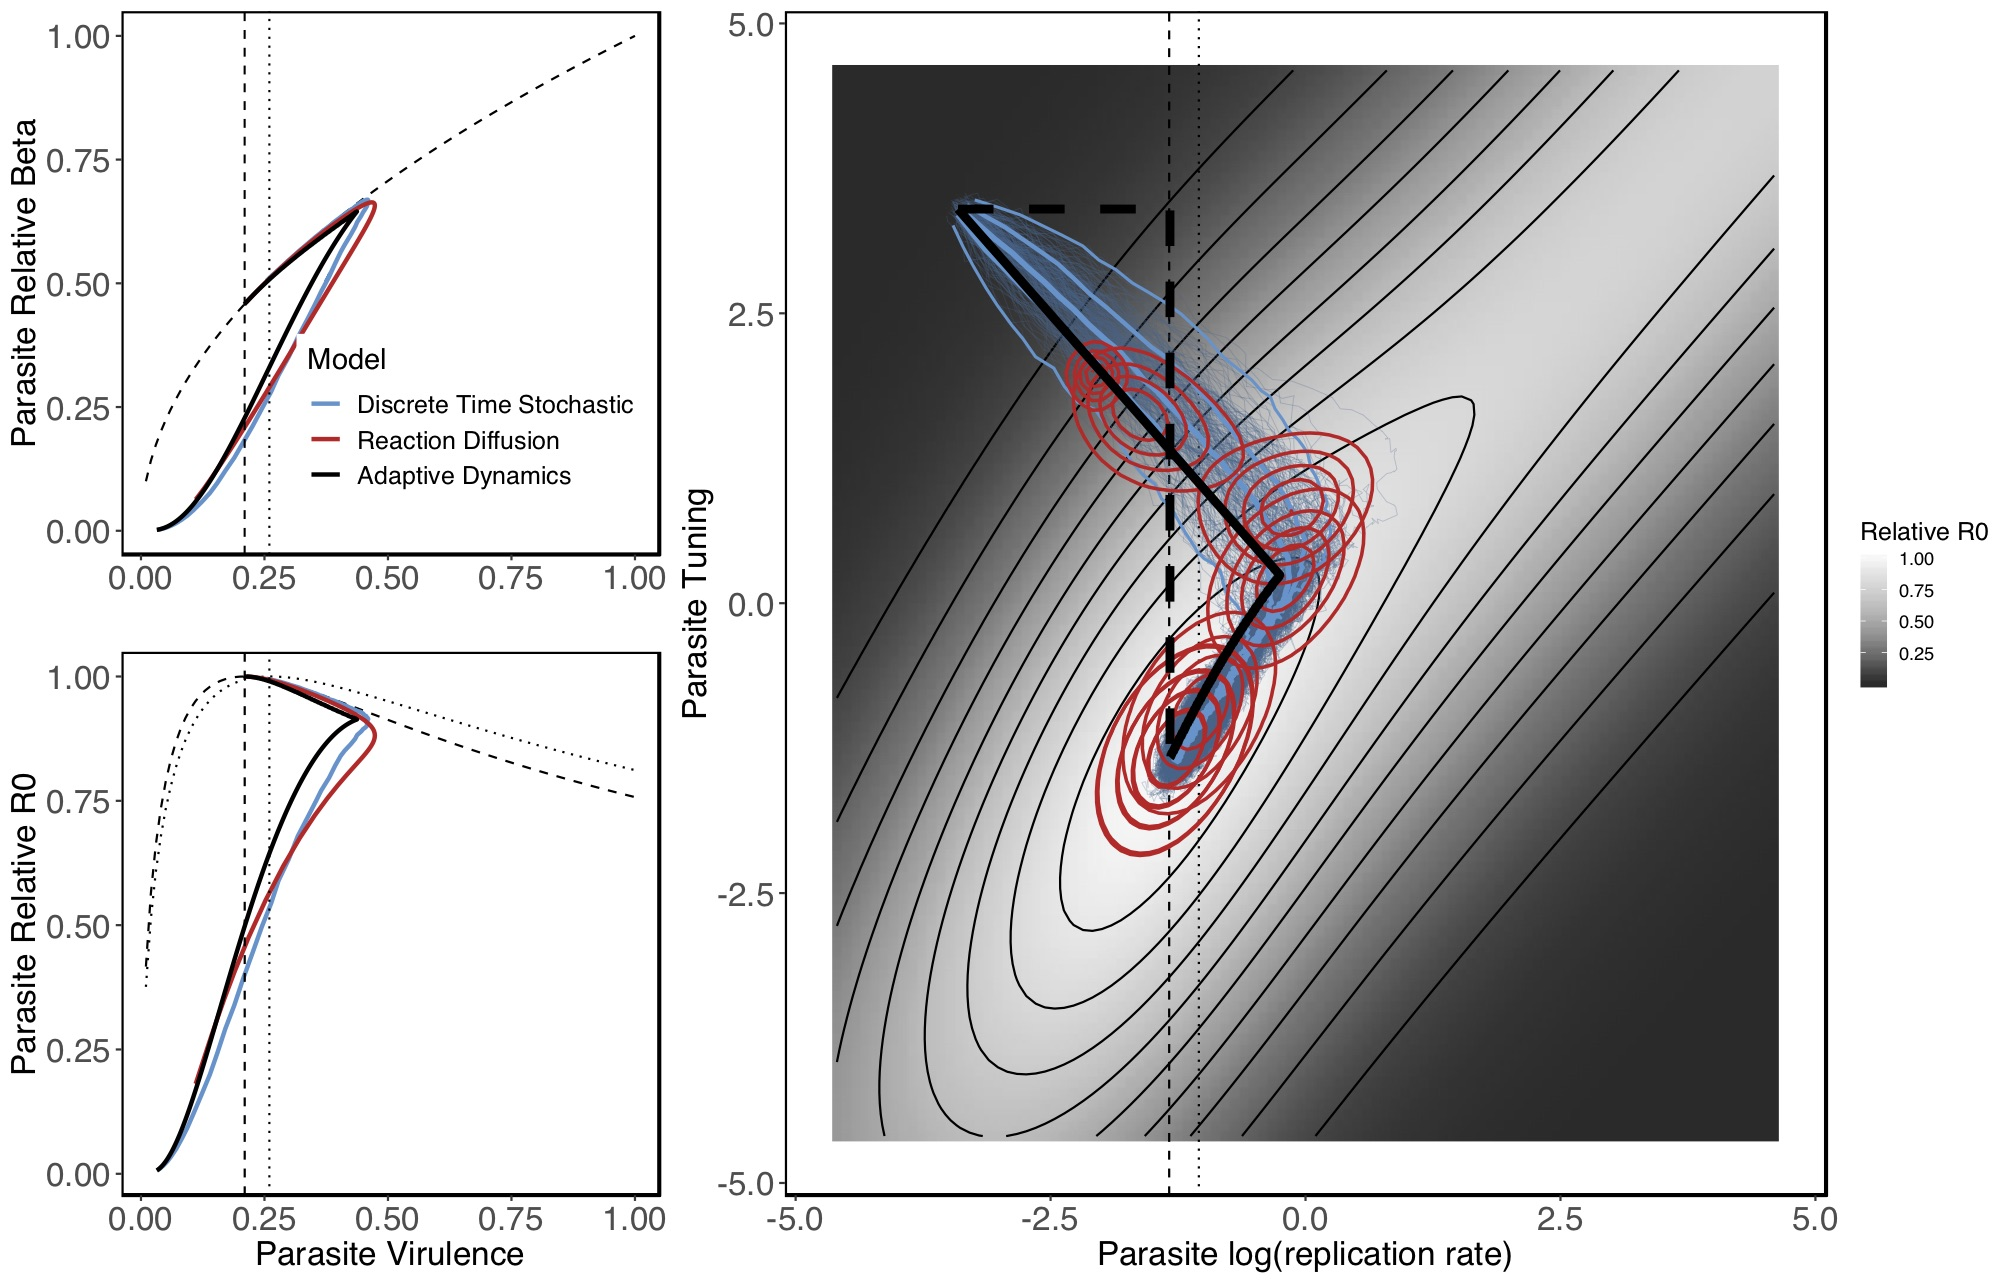
\includegraphics[width=1.0\textwidth]{Figures/landscape2.jpg}}
\caption{For a complete figure caption see \figref{landscape1}. Panels show the evolutionary trajectory of a parasite in the DTS (blue lines), RD (red ellipses), and AD (black solid and dashed lines) models, using the same parameter values as \figref{landscape1}, except with $\delta = 10$. A numeric summary of the DTS model for these parameter values is available in Table~2 row~8.} 
\label{fig:landscape2}
\end{figure} 
\clearpage

\clearpage
\begin{figure}[H]
\makebox[\textwidth][c]{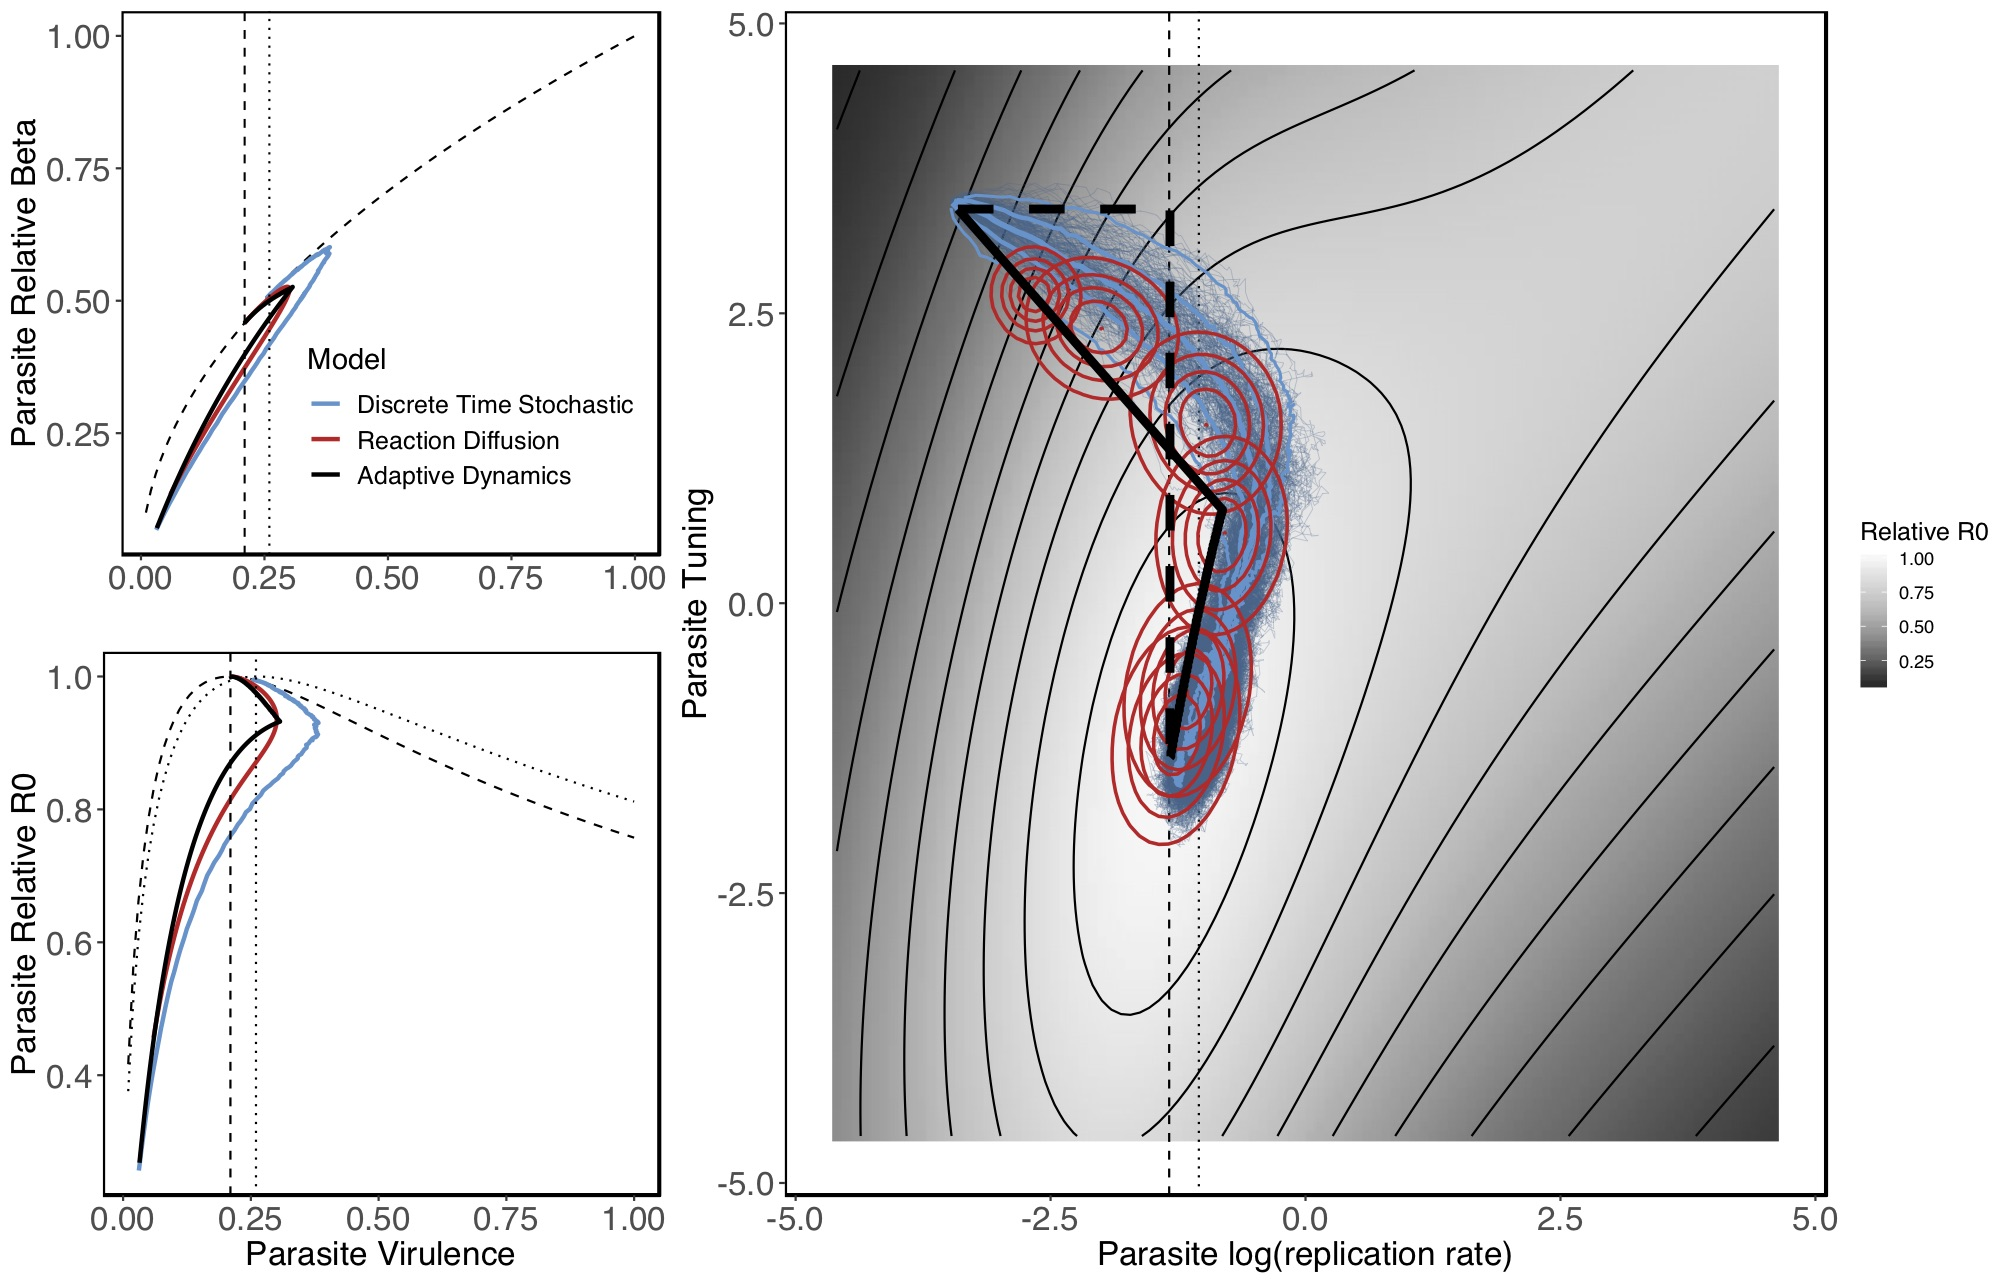
\includegraphics[width=1.0\textwidth]{Figures/landscape3.jpg}}
\caption{For a complete figure caption see \figref{landscape1}. Panels show the evolutionary trajectory of a parasite in the DTS (blue lines), RD (red ellipses), and AD (black solid and dashed lines) models, using the same parameter values as \figref{landscape1}, except with $\delta = 50$. A numeric summary of the DTS model for these parameter values is available in Table~2 row~9.} 
\label{fig:landscape3}
\end{figure} 
\clearpage

\subsection*{Parameter dependence: focus on the DTS model}

For each of our metrics of interest we find that a single parameter is the dominant source of variation; other parameters contribute, but to a lesser degree. Mutational probability ($\mu$) (followed by population size, N) has the strongest effect on the number of circulating strains (results for each of our model outcomes are shown in Table~2). The time it takes for a parasite population to reach its adaptive peak is a decreasing function of both mutation probability and population size, and to a lesser degree mutational standard deviation ($\sigma$). Maximum transient virulence is very consistent across parameters except for efficiency scale ($\delta$); decreasing $\delta$ results in lower transient virulence (Figures~1-3). The total time a parasite circulates while above optimum virulence is primarily a function of time to optimum virulence, and therefore is the largest for low mutation probability, low mutational standard deviation, and a smaller population size. Finally, departure from optimum virulence is driven almost entirely by population size. A smaller population size leads to a larger stochastic departure from the adaptive peak. For example, in Table~2, last column, row~3, the value of 0.17 means that $\sim$ 95\% of the 39 circulating strains (column~1 of "Model Outcomes") had a virulence between 0.20 and 0.33.

All of the results presented in Table~2 can be visualized in \figref{DTS1} except for the number of circulating strains. For parasite evolution from high replication rate and low efficiency see Figure~S1; for evolution from low replication rate, high efficiency see Figure~S2.

\clearpage
\begin{landscape}
\begin{table}[H]
\caption{Results for each of our model outcome for a subset of the parameter values presented in Table~1. The right half of the table lists results for the parameter values listed on the left. To improve presentation, parameter values are listed sparsely: for a given focal parameter, parameter values for all other parameters are constant. For example, in rows 1-3, parameter values for $\sigma$, N, and $\delta$ follow row 1. Model outcome columns, in order from left to right, are as follows: 1) Median number of circulating strains over the whole simulation; 2) Time (steps) to first reach optimum virulence, which can be roughly translated to a number of host generations by dividing by 100 (average life span of an uninfected host); 3) Maximum virulence reached during the evolution of the parasite to its adaptive peak; 4) Total time period where the parasite has a higher-than-optimum virulence; 5) Departure from optimum virulence lists the standard deviation in log(replication rate) (virulence on the logit scale) among circulating strains (median among all stochastic simulations) after optimum virulence is reached.} \label{tab:model_details} 
\resizebox{\columnwidth}{!}{
\bgroup
\begin{tabular}[t]{|R{2.50cm}:R{2.50cm}:R{2.50cm}:R{2.50cm}:R{2.50cm}|R{2.50cm}:R{2.50cm}:R{2.50cm}:R{2.50cm}:R{2.50cm}|}
\hline
\multicolumn{5}{|c}{\cellcolor[HTML]{EFEFEF} Parameters} & \multicolumn{5}{|c|}{\cellcolor[HTML]{9B9B9B}Model Outcomes}
\\
\hline
\cellcolor[HTML]{EFEFEF} \textbf{Focal Parameter}                &
\cellcolor[HTML]{EFEFEF} \textbf{Mutation Probability: $\mu$}    &
\cellcolor[HTML]{EFEFEF} \textbf{Mutational SD: $\sigma$}        &
\cellcolor[HTML]{EFEFEF} \textbf{Population Size: N} 		     & 
\cellcolor[HTML]{EFEFEF} \textbf{Efficiency Scale: $\delta$}     &     
\cellcolor[HTML]{9B9B9B} \textbf{Median number of circulating strains:} &
\cellcolor[HTML]{9B9B9B} \textbf{Time to optimum virulence:}           &
\cellcolor[HTML]{9B9B9B} \textbf{Maximum transient virulence:}   &
\cellcolor[HTML]{9B9B9B} \textbf{Time with greater than optimum virulence:} &
\cellcolor[HTML]{9B9B9B} \textbf{Departure from optimum virulence:}

\\
\hline 
             & 
0.001        &
0.05         &
600          &
30           &
3            &
$>$ 5x10\textsuperscript{5}  &
0.41         &
4.6x10\textsuperscript{5}    &
-- 
       
\\

$\mu$        & 
0.005        &
             &
             &
             &
11           &
1.1x10\textsuperscript{5} &
0.40         &
1.0x10\textsuperscript{5} &
0.14
       
\\

             & 
0.025        &
             &
             &
             &
39           &
3.4x10\textsuperscript{4}   &
0.40         &
3.0x10\textsuperscript{4}   &
0.17

\\
\hdashline

$\sigma$     & 
0.005        &
0.01         &
600          &
30           &
11           &
$>$ 5x10\textsuperscript{5} &
0.41         &
3.1x10\textsuperscript{5}   &
--
       
\\

             & 
             &
0.25         &
             &
             &
11           &
1.1x10\textsuperscript{4}   &
0.40         &
1.0x10\textsuperscript{4}   &  
0.21

\\
\hdashline

N            &
0.005        &
0.05         &
200          &
30           &
4            &
3.6x10\textsuperscript{5}   & 
0.41           &
3.3x10\textsuperscript{5}   &   
0.23
      
\\

             &
             &
             &
1800         &
             &
33           &
6.7x10\textsuperscript{4}   & 
0.41           &
6.0x10\textsuperscript{4}   &   
0.11 

\\
\hdashline

$\delta$     & 
0.005        &
0.05         &
600          &
10           &
11           &
1.7x10\textsuperscript{5}   & 
0.47          &
1.7x10\textsuperscript{5}   &   
0.09 
       
\\

             &
             &
             &
             &
50           &
11           &
1.3x10\textsuperscript{5}   & 
0.38         &
1.2x10\textsuperscript{5}   &   
0.18 

\\

\hline

\end{tabular}
\egroup
}
\end{table}

\clearpage

\end{landscape}
\clearpage
\begin{figure}[H]
\makebox[\textwidth][c]{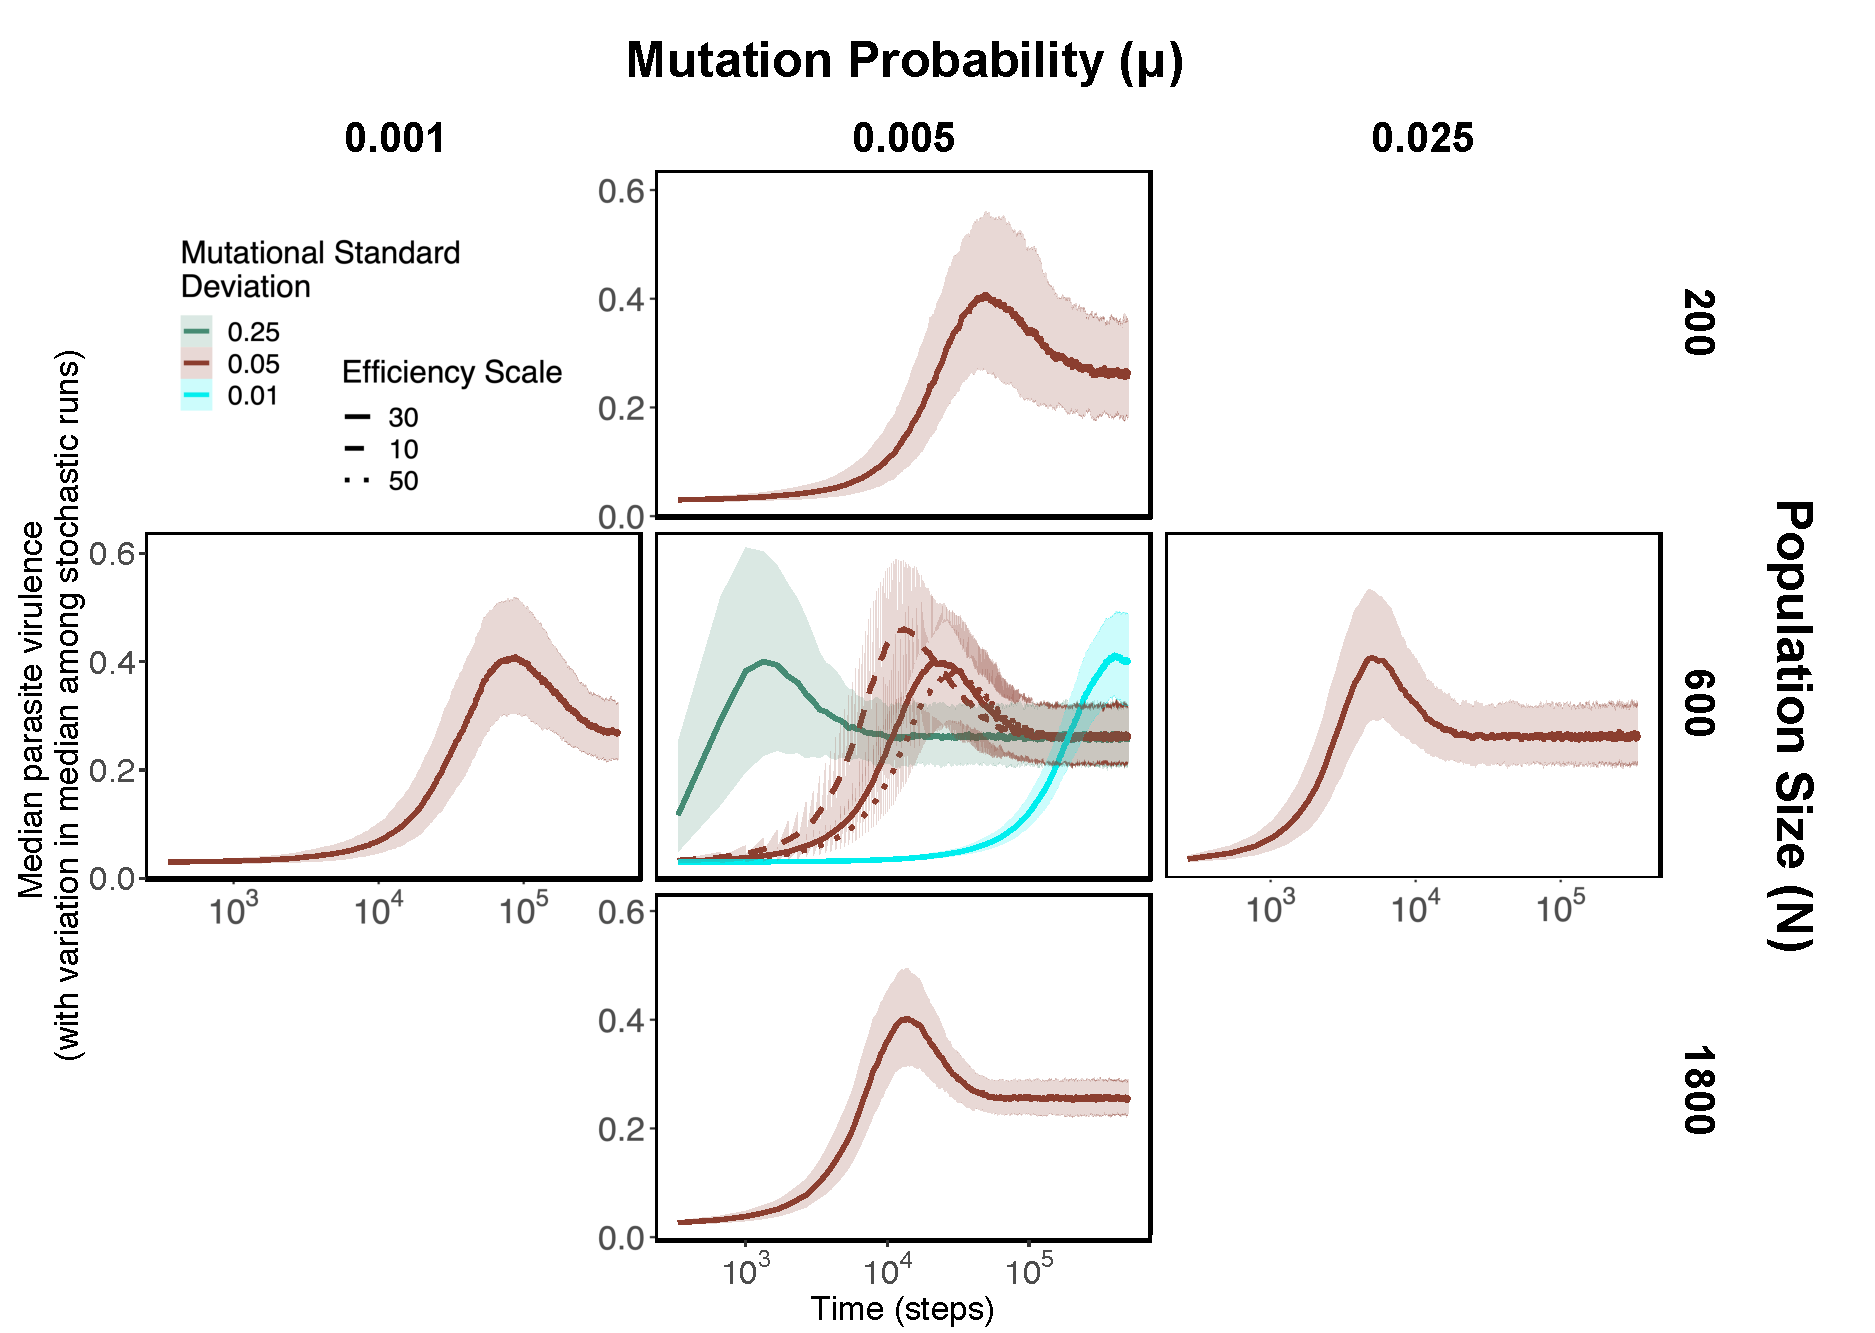
\includegraphics[width=1.0\textwidth]{Figures/DTS_results1edited.pdf}}
\caption{Parasite virulence for all parameter combinations presented in Table~2. Bold lines represent medians across 250 stochastic simulations; shaded envelopes show 95\% quantiles. The correspondence between the model outcomes presented in Table~2, from left to right, are as follows: 1) Median number of circulating strains: not pictured; 2) Time to optimum virulence: Time at which median virulence first reaches 0.26; 3) Maximum transient virulence: maximum of each curve; 4) Time with greater than optimum virulence: width of the peak; 5) Departure from optimum virulence: not \emph{directly} pictured. The width of the shaded envelope shows the variation in median virulence among stochastic simulations, not the median among all stochastic simulations for standard deviation in virulence among circulating strains within each simulation, which is what Table~2 shows. However, because all simulations converge on a virulence of 0.26, there is a strong correlation between these two metrics; the width of the shaded envelope after the parasite population reaches a median of 0.26 follows the same \emph{pattern} as the numbers presented in the Table~2, but are not quantitatively identical.} 
\label{fig:DTS1}
\end{figure} 
\clearpage

We present an expanded center panel from \figref{DTS1} in \figref{DTS2}. This plot shows each of the 250 stochastic simulations for the first three rows of Table~2; the center red curve is the result presented in \figref{landscape1} (only an efficiency scale of 30 is pictured in \figref{DTS2}). This plot also shows the median and 95\% density for the virulence of the parasite strains in the RD solution, which is similar to the stochastic simulation result. The optimum virulence of 0.21 for the RD model and 0.26 for the DTS model are seen here.

\begin{figure}[H]
\makebox[\textwidth][c]{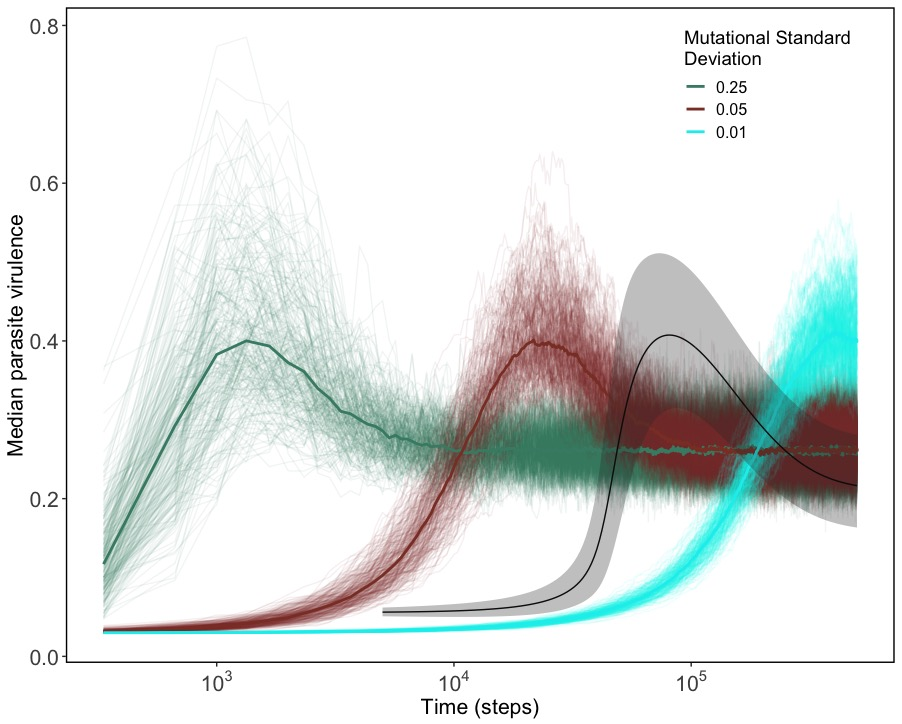
\includegraphics[width=1.0\textwidth]{Figures/DTS_results_zoomed.jpeg}}
\caption{Parasite median virulence and virulence across all stochastic simulations for the center panel of \figref{DTS1} with only $\delta = 30$ shown (these parameter combinations are also shown in \figref{landscape1} and in the first three rows of Table~2). The solid black curve and shaded grey envelope show the median and 95\% density for the virulence of the parasite strains in the RD solution.} 
\label{fig:DTS2}
\end{figure} 
\clearpage

\section*{Discussion}

Previous work assuming a tradeoff between virulence and transmission has shown that evolution on ecological timescales, for example during an epidemic, selects for strains with higher instantaneous growth (little r) more strongly than for strains with higher $\rzero$ \citep{DayandProulx2004, Bolkeretal.2010}. Eco-evolutionary feedbacks can be seen here in the comparison between AD and RD/DTS solutions in \figref{landscape1} and Figure~S2, though our model also provides a new mechanism in addition to eco-evo dynamics for why a pathogen may evolve higher transient virulence: parasite tuning selects for higher virulence in the short term when a parasite evolves from an initial position of low virulence and low efficiency. A larger cost of a mismatch between virulence tuning (which lowers $\beta$ at a given level of $\alpha$) leads to very high transient virulence (\figref{landscape2}). When scaled to host lifespan in the absence of infection, the transient virulence period pictured in \figref{landscape2} represents 1,600 host lifespans. While this is unrealistic for any vertebrate host, it may be an appropriate time scale for viral parasites of algae \citep{Frickeletal.2016, Frickeletal.2018} or bacteria \cite{Berngruberetal.2015}.

When a parasite evolves from high virulence and low efficiency, another plausible scenario for an emerging pathogen, all three models agree that a parasite evolves monotonically to its optimum. However, the length of time that it takes for a parasite to reach its optimum virulence increases as the fitness impact of tuning increases (e.g. as $\delta$ decreases). The evolutionary distance covered by a parasite evolving directly to its optimal virulence reflects evolution only \emph{on} the tradeoff curve; this distance is shown in the horizontal portion of the bold dashed line in Figure~S1. Collectively, these results show that in the simple case of a fitness landscape with a single global maximum AD, RD, and DTS models agree on the general trajectory of parasite evolution. With a multi-peaked surface, however, AD solutions may not agree with the RD or DTS solutions \citep{Dieckmann2002}. For example, when a local maximum exists with a steeper gradient, AD models can show that a parasite resides at this local maximum indefinitely. Diffusion in RD and DTS models allow populations to evolve through fitness valleys, which has been documented empirically \citep{JainandJoachim2007, Gokhaleetal.2009, Weissmanetal.2010}. This scenario requires more detailed analyses than those presented here.

Despite the similarities between the RD and DTS model solutions, the dynamics we plot reflect slightly different processes. The RD model reveals variation within a population of parasites, while the DTS model solution represents variation among stochastic realizations. While we do not show them here (and only report variation after equilibrium is reached--Table~2 last column), simulation results show that with similar parameter values for $\sigma$ in the RD and DTS model, population level variation in the RD model is about an order of magnitude larger than in the DTS model. Approximately an order of magnitude smaller value for $\sigma$ in the RD model is needed for roughly similar estimates of within-population variation.

If general qualitative patterns are of primary interest, a RD model is likely preferable to a DTS model because it is easier to implement and faster to solve. However, while RD and DTS models (and under many starting conditions the AD model) broadly agree on qualitative dynamics, it is important to keep in mind that these models generate slightly different landscapes shapes for the same numeric values for host recovery and host background death rate. The even simpler AD model used here provides a description of gradient ascent (tracking the steepest path up the landscape), which can provide a description of the final evolutionary state of the system (as long as careful attention is paid to the muli-peakedness of the landscape), but may underestimate transient dynamics. If rare evolutionary events in small populations are of primary interest, only the DTS model can provide an adequate estimate. It is also important to keep in mind however, that with any more complicated of a model than is used here, for example with host evolution in defense traits, the number of differential equations in the RD model becomes unwieldy and solving this system can take longer than solving the DTS model. 

For the DTS model specifically, results were as expected. An increase in population size minimized the effects of stochasticity, decreased the time to optimal virulence, and decreased a populations departure from optimum virulence. Both a larger mutation probability and mutational standard deviation decrease time to equilibrium and increase transient departure from equilibrium. The transient virulence peak is determined mostly by the shape of the fitness landscape, with an increase in the cost of a mismatch between replication rate and tuning increasing transient virulence.

\subsection*{Caveats and model extensions}

Despite our breadth of coverage of methods for solving our model, we considered only an SIS type  epidemiological model, which does not allow for recovered hosts that are permanently immune to infection (e.g. an SIR model), despite lifetime immunity in many wildlife diseases (e.g. WNV, MYXV). We also ignore variation in host recovery across parasite strains, even though tradeoff between host recovery and parasite virulence can also constrain parasite exploitation strategy \citep{Alizon2008}. It would be interesting to extend our model an SIR model with recovered hosts of incomplete and waning immunity as seen in \emph{Mycoplasma gallisepticum} infection of House Finches \citep{Flemingetal.2018}. In this system incomplete and waning immunity favors the evolution of more virulent strains which are able to overwhelm a hosts incomplete immunity. However, these evolutionary patterns are not yet fully understood. With a small extension to explicitly consider host defense, our model for secondary trait evolution could help to explain the evolution of virulence in this system. 

We also define host-parasite interactions using only a quantitative genetic model, though many host-parasite systems (e.g. flax-flax rust: \citealt{IslamandShepherd1991}, human/bird-influenza: \citealt{Smithetal.2004, PoullainandNuismer2012}, \emph{Pseudomonas fluorescens} and its DNA phage: \citealt{Poullainetal.2008}) can arguably be better understood using a more explicit gene based approach. A matching allele model (MA), for example, assumes that a perfect match between host and parasite genotype is required for infection, while a gene-for-gene (GFG) model relaxes these assumptions slightly, allowing for a decay in infection success as a function of increasing genetic distance \citep{AgrawalandLively2002, NuismerandOtto2005, Thralletal.2016}. Often these models are usually analyzed in a co-evolutionary framework, and have shown to lead to evolutionary cycles such as Red-Queen dynamics \citep{Decaesteckeretal.2007}. In the absence of host evolution, our quantitative genetic model has a clear parallel to a GFG model, with tuning serving as a form of genetic distance, and transmission as a measure of infection success. However, to fully realize the connection between these models it is necessary to extend our model to allow for host evolution.

For the model that we do examine, a few of our assumptions could be explored/relaxed in order to cover a wider range of possible dynamics. First, we assume a very strong form of density dependent birth that greatly reduces the probability of population extinction (e.g. with N = 200 none of populations in the 250 simulations went extinct, though with populations of 100, extinction probability was roughly 10-20\%). Given our focus here on a parasites' evolutionary path to their global optimum and the size of the departure from optimum virulence, we chose population sizes to minimize extinction. It will be important to examine the starting conditions that make it unlikely a parasite would escape extinction; these are likely dead end hosts for the parasite. Given our strong assumption for density dependent birth, it is possible that the results we present here are modeling an unrealistic scenario of a pathogen evolving to exploit what is in reality an unsuitable host.

Second, while our assumption of mutational effects on a logistic scale is logical, mutation on one scale and selection on another has the potential to produce very odd dynamics. For example, mutation on the log scale and selection on the linear scale can leads to exponentially increasing fitness, albeit in the absence of tradeoffs. Regardless, it may be fruitful to examine mutation and selection on the same scale in order to understand what portion of the dynamics we see are due simply to our modeling choices. 

Finally, as mentioned previously we assume a static, homogeneous host population, which is an unrealistic assumption for any host population. A vast literature exists for a static, heterogeneous host population which shows that host heterogeneity has a large influence on parasite optimum virulence (e.g. \citep{EbertandHamilton1996, Gandonetal.2001, Ganusovetal.2002, Gandon2004, Kainetal.2018}). When host populations evolve with parasite populations, evolutionary cycles and stable polymorphisms can occur \citep{CarvalandFerriere2010, Bestetal.2014, Athanasiadouetal.2015}. In order to make our model more realistic it will be important to extend our model to consider the evolution of host resistance (reducing parasite load) and tolerance (decreasing fitness costs for a given pathogen load) on ecological time scales (for reviews on resistance and tolerance see \citealt{SchneiderandAyres2008, AyresandSchneider2012, KutzerandArmitage2016}). 

